\documentclass[a4paper, 11pt]{article}
\usepackage[utf8]{inputenc}
\usepackage{graphicx}
%\usepackage{amsfont}
\usepackage{amsmath}
\usepackage{amssymb}
\usepackage{hyperref}
%\usepackage[french]{babel}

\begin{document}

\title{Moteur de lancer de rayons}
\author{Coiffier Guillaume - Béthune Louis - Felderhoff Joël}
\date{Janvier 2017} 

\maketitle

\section*{Présentation (cf Wikipedia)}
 
Le \textit{Raytracing} (ou lancer de rayons en québecois supérieur) est une méthode de rendu de scènes 3D. Il permet d'obtenir des images d'excellente qualité en simulant le comportement naturel de la lumière : réflexions, ombres, changement d'indice, diffusion, éclairage, flou de profondeur... 
  
La théorie sur le domaine est assez ancienne (années 60) mais l'exigence de cette méthode en terme de charge de calcul ont longtemps limité son usage. Cette technologie a donc connu une renaissance dans les années 2000, notamment dans le cinéma d'animation ou la simulation scientifique.  
  
C'est une technique assez simple à mettre en œuvre et on obtient rapidement des résultats, même si un moteur complet (comme celui ayant produit l'image ci-dessous) nécessite un travail titanesque.

\begin{center}
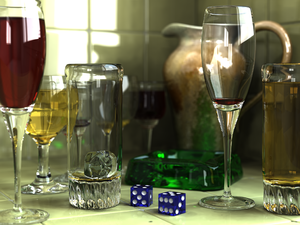
\includegraphics[scale=1]{300px-Glasses_800_edit.png}
\end{center}
\newpage

\section{Principe}
L'idée est de simuler le comportement d'un rayon lumineux, en utilisant le principe du parcours inverse de la lumière.  
  
Ainsi, pour chaque pixel de la caméra, on lance un rayon et on cherche le premier objet qu'il intersecte. On peut alors afficher ce pixel de la couleur de l'objet. 
  
\begin{center}
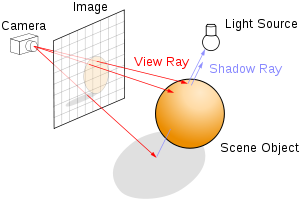
\includegraphics[scale=0.8]{300px-Ray_trace_diagram.png} 
\end{center}

On peut prendre en compte l'éclairage de façon très simple : on calcule les coordonnées du point d'intersection, puis on "tire" un rayon imaginaire en direction de la source de lumière. Si ce rayon atteint la source de lumière, le pixel apparaît éclairé. Dans le cas contraire, si on intersecte un autre objet de la scène, alors il y a occlusion et le pixel apparaît en sombre.  

\begin{center}
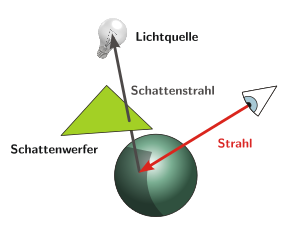
\includegraphics[scale=0.8]{290px-Raytracing-Schattenstrahl.png} 
\end{center}  
Par la suite vous pouvez facilement simuler des dispositifs optique devant la caméra comme une lentille pour produire des effets...  
\newpage

\section{Votre mission}
\subsection*{Niveau 1 : le z-buffer}

Implémentez un raytracer élémentaire. Pour cela vous devez supporter :  
  
\begin{description}
\item [Une caméra] simple unidirectionnelle, de normale orientée selon l'axe z et centrée en $(0, 0, 0)$
\item [Des objets simples] comme des sphères monochromatique. Pensez à une architecture assez souple pour pouvoir gérer d'autres formes plus tard. 

Équation décrivant un rayon : $ t\in \mathbb{R}, d\in \mathbb{R}^3, O + dt$ où $d$ est la direction
 
Équation décrivant une sphère : $(x - x_0)^2 + (y - y_0)^2 + (z - z_0)^2 = R^2$ de centre $(x_0, y_0, z_0)$ et de rayon $R$
\item [Un z-buffer] pour prendre en compte la profondeur. Les objets proches doivent être affichés avec des couleurs vives, et les objets lointains avec des couleurs sombres. 
  
\end{description}  

\subsection*{Niveau 2 : d'autres formes et des couleurs}

Rajoutez :

\begin{description}
\item [D'autres formes] comme des triangles par exemple. Intéressez vous à l'algorithme de \textit{Moller Trumbore}.  
\item [De la couleur] sur vos objets. Prévoyez une architecture assez souple pour gérer des matériaux plus compliqués plus tard (surfaces réfléchissantes, textures).  
  
\end{description}  

\textbf{Exemple :}
  
\begin{center}
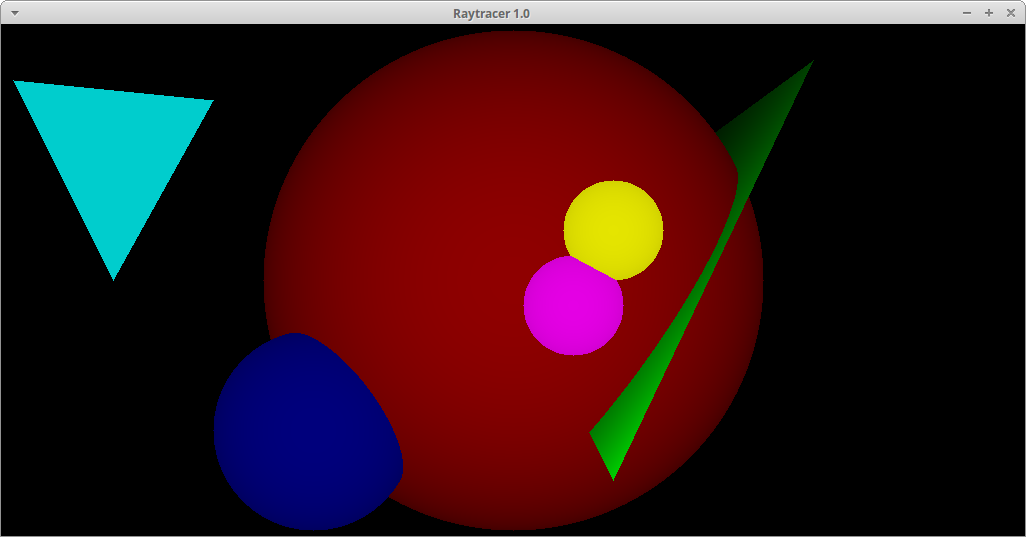
\includegraphics[scale=0.25]{correct1.png} 
\end{center}

\subsection*{Niveau 3 : ambient occlusion}

Rajoutez un système plus réaliste plus réaliste qui remplacera le z-buffer : à présent la luminosité dépend de l'angle avec lequel la lumière arrive sur l'objet. Vous pouvez considérer dans ce modèle simplifié que votre caméra et la source de lumière sont confondus.  
  
Lorsque le rayon intersecte la surface d'un objet, déterminez l'angle que ce rayon forme avec la surface. Si le rayon est normal à la surface la luminosité est maximale, et s'il est tangent la luminosité est proche de 0.  
  
Cela se comprend bien sur le schéma suivant :  

\begin{center}
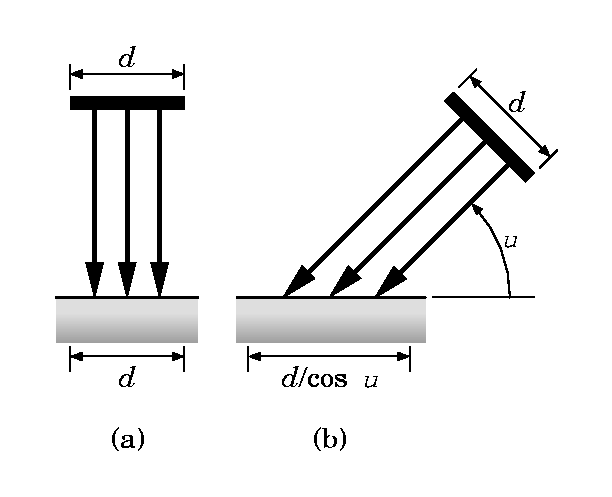
\includegraphics[scale=0.3]{an06f16.png} 
\end{center}  
  
Profitez en pour faire évoluer votre caméra : elle doit pouvoir être placé n'importe où avec des orientations différentes.  
  
  
\textbf{Exemple :}
  
\begin{center}
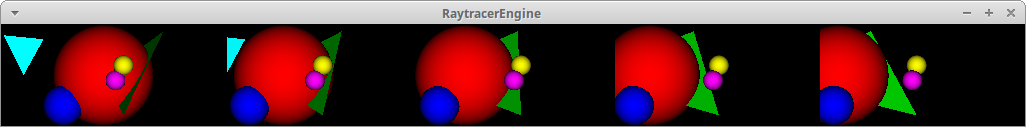
\includegraphics[scale=0.45]{multi-orientations.png} 
\end{center}

\subsection*{Niveau 4 : sources multiples et gestionnaire de fenêtres}

Ajoutez des sources de lumière à votre scène. Sources directionnelles ou isotropes. Sources blanches ou colorées (auquel cas vous réaliserez de la synthèse soustractive sur votre objet). Cela vous permettra de l'éclairer de différentes façons.  
  
Profitez en pour faire un gestionnaire de fenêtre, pour effectuer plusieurs rendus en parallèle d'en coup, chacun avec sa caméra (c'est pratique pour déboguer et comparer des images).  

\begin{center}
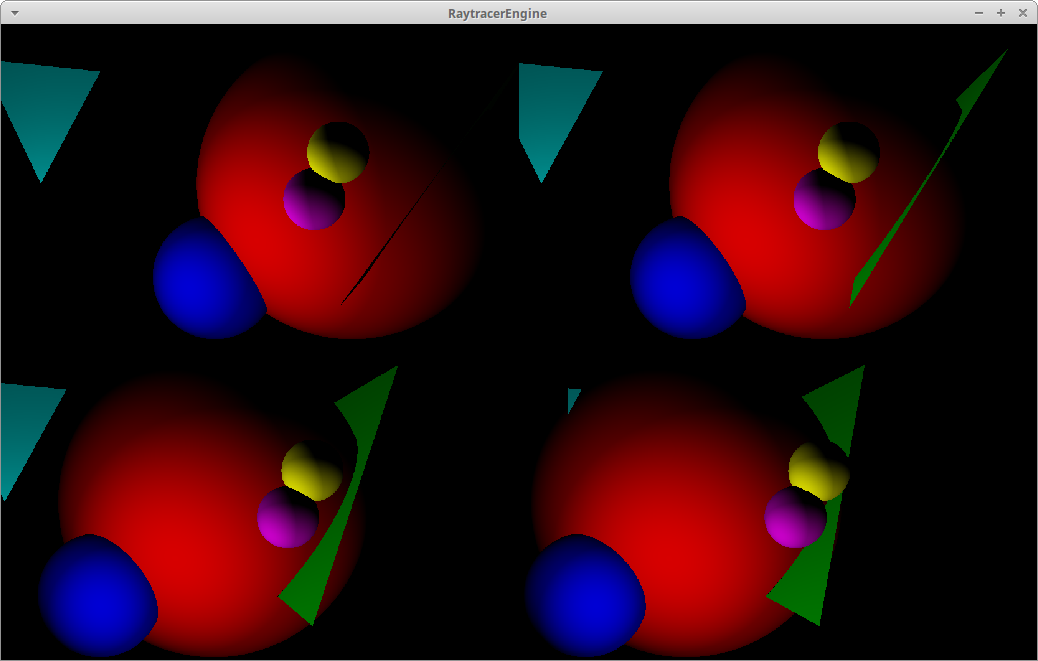
\includegraphics[scale=0.2]{window_manager4.png} 
\end{center}

\subsection*{Niveau 5 : scripting et formats de fichier}  
  
Vous allez avoir besoin de faire de plus en plus de tests. Il est malaisé de recompiler le programme à chaque changement (lorsque le cœur du moteur ne change pas, mais que vous modifiez le contenu de votre scène et les méthode de rendu). De plus vous pourriez vouloir vous faire un stock de différentes scènes.  
  
Il peut donc être intéressant de créer des fichiers servant à décrire une scène. Choisissez le format !  
  
\textbf{Exemple :}
  
\fontsize{9}{11}\selectfont
\begin{verbatim}
name=sphere
width=832
height=512
nb_objects=2
nb_displayer=1
layout=(1,1)

#CAMERAS

camera1:
 pos=(0,0,0)
 orient=(0.,0.)
 width=832
 height=512
 gammaWidth=1.
 gammaHeight=1.

#OBJECTS

objet1:
  type=Sphere
  center=(0,0,500)
  radius=250
  material=ColorGreen

light1:
  type=LampPoint
pos=(0,500,-200)

\end{verbatim}  
  
Ce n'est bien sûr qu'une suggestion. Notez que le travail de parsing est plus aisé avec un langage de script comme Python que C++. Ainsi c'est la bonne occasion pour écrire un peu de code dans le langage de script de votre choix, et interfacer ce langage avec C++. Dans le cas de C++ on s'intéressera à la bibliothèque Boost.Python (\url{http://www.boost.org/doc/libs/1_63_0/libs/python/doc/html/index.html}) ou même à la bibliothèque Boost en général qui propose de nombreux outils et algorithmes utiles pour toute sortes de projets.  
  

\subsection*{Niveau 6 : dans les étoiles}  
  
A l'heure où j'écris ces lignes, notre implémentation ne propose rien de plus que ce que présenté précédemment. Néanmoins vous pouvez rajouter les éléments suivants :  
  
\begin{itemize}
\item des textures
\item des surfaces réfléchissantes
\item du flou de profondeur
\item de l'antialiasing
\item etc... informez vous sur l'état de l'art
\item Stockez votre scène dans une structure de données performante (comme un arbre par exemple, qui partitionne votre espace).
\end{itemize}  
  
Essayez de faire ça :  
  
\begin{center}
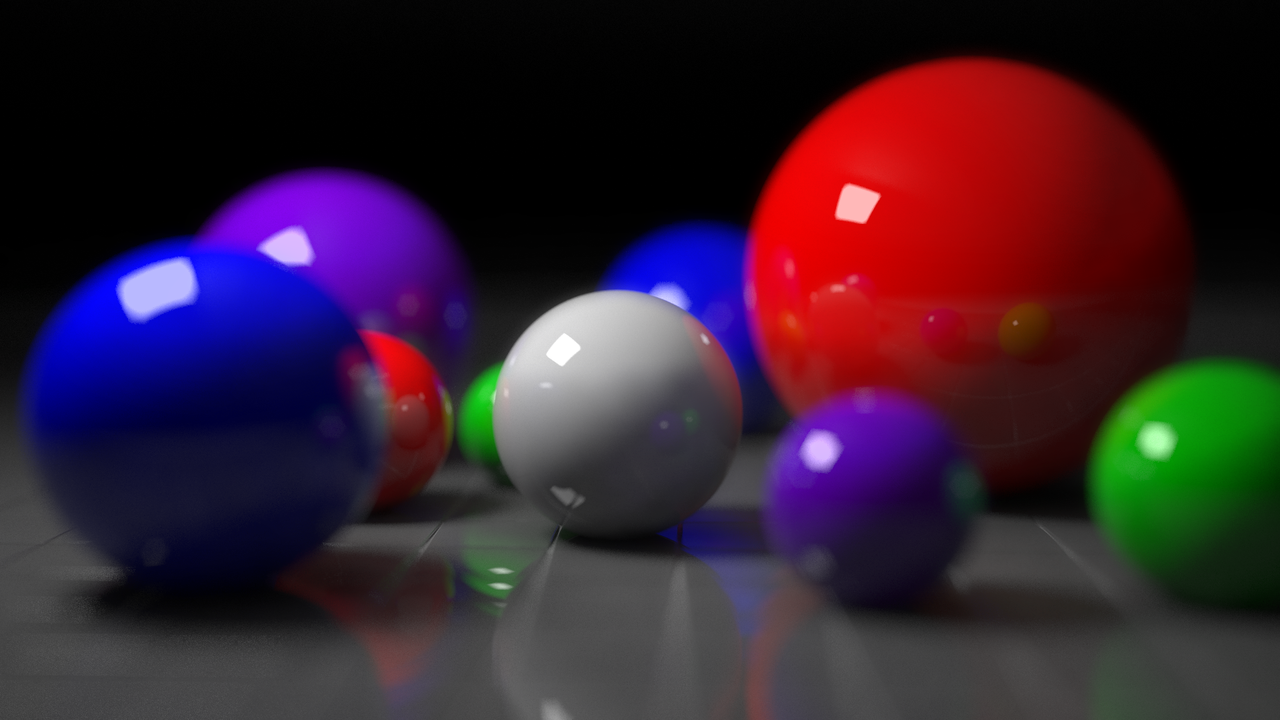
\includegraphics[scale=0.25]{1280px-BallsRender.png}  
\end{center}

\newpage
\section*{Conseils}  
\subsection{Architecture}  
  
Pensez que votre moteur va évoluer. L'idée est de mettre en pratique tout ce que vous avez appris en terme de programmation orientée objet et de généricité pour créer quelque chose adaptatif et évolutif.   
  
Pensez par exemple à une interface IForme pour vos différentes formes, et posez vous les questions suivantes : qu'est ce qui caractérise mon objet ? Quel interface doit-il offrir ? Si vous codez en vous posant ces questions, votre architecture ne peut que tendre vers le bon.  
  
Sachez qu'il n'existe pas de solution universelle, et seul un mélange d'essais/erreurs et d'expérience, couplé à de bonnes pratiques, peuvent mener à un résultat satisfaisant. Informez vous sur les \textit{designs patterns}.  

\subsection{Travail à plusieurs}
Autre chose : une solution pour travailler vite et avoir quelque chose de plus puissant est de travailler à plusieurs. Parlez en à votre TDman/TDgirl et profitez en pour apprendre à travailler à plusieurs sur un même code : regardez du coté de Git.

\subsection{Bibliothèque et langage}  
  
La bibliothèque standard du C++ ne propose pas nativement de moyens de faire du fenêtrage ou des applications graphiques. Il vous faudra donc une bibliothèque extérieure, dont il faudra apprendre la documentation et le fonctionnement.

Il en existe des dizaines mais je suggère à titre personnel la SFML(\url{https://www.sfml-dev.org/index-fr.php}) qui est :  
  
\begin{itemize}
\item simple à utiliser et très intuitive, peu volumineuse
\item suffisamment rapide pour l'usage que l'on va en faire
\item entièrement orientée objet
\item exploitant les mécanismes du C++ idiomatique comme la RAII
\item développée par un français, avec des tutoriels en français et une communauté francophone active
\item multi-plateforme
\end{itemize}

Essayez de faire du C++ idiomatique vous aussi : faites usage du polymorphisme pour une architecture plus souple. Faites un usage intensif de pointeurs intelligents (\textit{shared\_ptr} ou \textit{unique\_ptr}) pour vous prémunir des fuites de mémoire. 

\subsection{Bonjour je suis un malade mental}

Si après tout ça vous vous ennuyez encore, essayez d'obtenir un moteur performant.  
  Stockez votre scène dans une structure de données performante (comme un arbre par exemple, qui partitionne votre espace).
Faites des benchs. Parallélisez vos boucles. Refaites des benchs. Lancez plein de threads. Rerefaite des benchs. Réécrivez tout pour avoir un code qui profite du cache.  
  
Décidez que vous êtes meilleur que votre compilateur et écrivez de l'assembleur pour les parties critique du code. Faites des benchs. Abandonnez cette idée de merde.  
  
Regardez du côté du calcul GPU (par exemple avec CUDA ou OpenCl) pour profiter des quelques mille cœurs de calcul que votre carte graphique met aimablement à votre disposition.     
\end{document}
